\documentclass{article}
\usepackage{graphicx} % Required for inserting images
\usepackage{graphicx} % Required for inserting images
% Change page dimensions
\usepackage[margin=1in]{geometry}
\usepackage{amsmath}
\usepackage{amssymb}
\usepackage{subcaption} % in preamble
\usepackage{algorithm}
\usepackage{algpseudocode}
\usepackage{minted}
\usemintedstyle{friendly} % or bw, colorful, etc.

\title{AMIC Uncertainty – Monte Carlo Method}
\author{Leon King}
\date{August 2025}

\begin{document}

\maketitle

\section{Introduction}
AMIC is a language model that can integrate self-attention neural network models with logistic regression methods to analyze sentiment. However, the current architecture of AMIC can only provide point estimation in either continuous regression or classification. As a statistician, I always want to know the uncertainty level about the point estimation. So this is why we would like to modify AMIC to produce a confidence interval more like a statistic.

\section{Methods}
There are two major ways to employ uncertainty in the AMIC model. One way is quick and straightforward, but less accurate. It is to add a dropout layer to the AMIC model, then repeat the forward pass of the model to generate a sample of predictions. Finally, the mean, variance, lower quantile, and upper quantile can be calculated from these Monte Carlo samples. Another approach is a more complicated but more accurate method for calculating uncertainty based on the Variational Bayesian. The method is to add one Bayesian layer to the model.  

\section{Monte Carlo Method}
In the class of Synthesizer, which is the final building block of the AMIC model, it has a dropout layer with a probability of 0.2 in the forward pass. After full training, we would run each review on the trained Synthesizer module to generate Monte Carlo samples using this dropout layer. 

\section{Code Snippet}
The following algorithm displays how the samples are drawn and summary statistics are calculated for each review. 
\begin{algorithm}[!ht]
\caption{MC Dropout Inference for AMIC}
\label{alg:mc-dropout}
\begin{algorithmic}[1]
\Require model with dropout, inputs $(\text{sent}, \text{digits}, \text{mask})$, samples $T$
\State Activate dropout at inference: \texttt{model.train()}
\For{$t=1$ to $T$}
  \State $\hat{y}^{(t)} \gets \text{model}(\text{sent}, \text{digits}, \text{mask}, \text{use\_mask})$
\EndFor
\State $\bar{y} \gets \frac{1}{T}\sum_{t=1}^T \hat{y}^{(t)}$, \quad
$s^2 \gets \frac{1}{T-1}\sum_{t=1}^T(\hat{y}^{(t)}-\bar{y})^2$
\State \Return $\{\hat{y}^{(t)}\}_{t=1}^T$, $\bar{y}$, $s^2$
\end{algorithmic}
\end{algorithm}

The following code Snippet in Python displays the exact detailed code to realize this simple Monte Carlo Uncertainty. The key argument to this mc\_dropout\_predict() is the model and T. The model we used here is Synthesizer. Other classes also have dropout layers. Eventually, we can take advantage of each class's dropout layer to generate samples based on the entire architecture. T refers to the number of samples we want for each observation. Here I set it up to 50, but we can set it up to more samples. 
\begin{listing}[!ht]
\caption{Monte Carlo Dropout prediction wrapper for AMIC/Synthesizer.}
\label{lst:mc-dropout}
\begin{minted}[fontsize=\small, breaklines, linenos]{python}
def mc_dropout_predict(
    model: torch.nn.Module,
    sent: torch.Tensor,
    digits: torch.Tensor,
    mask: torch.Tensor,
    use_mask: bool = False,
    T: int = 50,
    device: torch.device = None
):
    if device is None:
        device = next(model.parameters()).device
    sent   = sent.to(device)
    digits = digits.to(device)
    mask   = mask.to(device)

    # Enable dropout at inference
    model.train()

    # collect T predictions
    preds = []
    with torch.no_grad():
        for _ in range(T):
            sig_out, _, _ = model(sent, digits, mask, use_mask=use_mask)
            preds.append(sig_out)        # each sig_out: (batch_size,)

    # stack to (T, batch_size)
    preds = torch.stack(preds, dim=0)

    # posterior mean and variance
    mean_pred = preds.mean(dim=0)     # (batch_size,)
    var_pred  = preds.var(dim=0)      # (batch_size,)

    return preds, mean_pred, var_pred
\end{minted}
\end{listing}

\paragraph{Monte Carlo summary statistics.}
Given a set of $T$ Monte Carlo samples $\{ s_t \}_{t=1}^T$ from the model’s predicted probabilities:

\begin{align}
\text{Posterior mean:} \quad
\bar{p} &= \frac{1}{T} \sum_{t=1}^{T} s_t, \\[6pt]
\text{Posterior variance:} \quad
\sigma_p^2 &= \frac{1}{T} \sum_{t=1}^{T} (s_t - \bar{p})^2, \\[6pt]
\text{95\% credible interval:} \quad
\mathrm{CI}_{95\%} &= \big[\, Q_{2.5}(s),\; Q_{97.5}(s) \,\big], \\[6pt]
\text{Empirical class probability (class 1):} \quad
\hat{P}(y=1) &= \frac{1}{T} \sum_{t=1}^{T} \mathbb{I}[\,s_t > 0.5\,], \\[6pt]
\text{Empirical class probability (class 0):} \quad
\hat{P}(y=0) &= 1 - \hat{P}(y=1), \\[6pt]
\text{Predicted label (mean threshold):} \quad
\hat{y} &= \mathbb{I}[\,\bar{p} > 0.5\,], \\[6pt]
\text{Certainty flag:} \quad
\mathrm{certain} &= \big(\; Q_{2.5}(s) > 0.5 \;\big) \;\lor\; \big(\; Q_{97.5}(s) < 0.5 \;\big),
\end{align}

where $Q_{\alpha}(s)$ denotes the $\alpha$th percentile of the sample set and $\mathbb{I}[\cdot]$ is the indicator function.




\section{results}
The final table from the train dataset would look as follows:
\begin{figure}
    \centering
    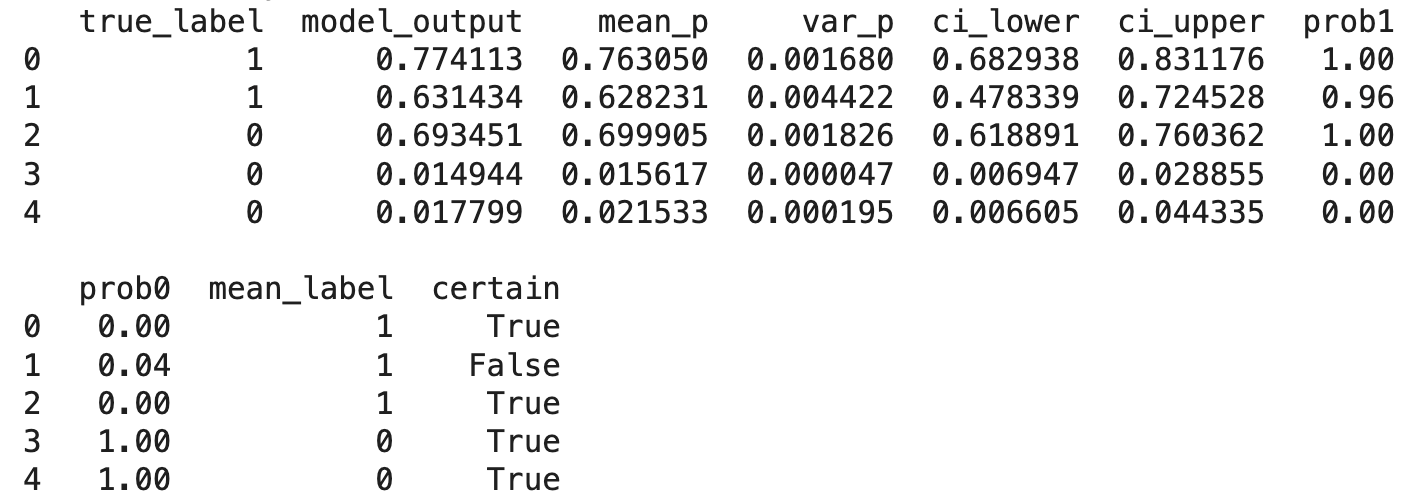
\includegraphics[width=0.7\linewidth]{table.png}
    \caption{Uncertainty Table}
    \label{fig:placeholder}
\end{figure}
If the lower confidence interval limit is greater than 0.5, the probability of being class 1 would be 1. If the upper confidence limit is less than 0.5, the probability of being 0 would be 0. If the 95\% confidence interval contains the 0.5, then the frequency of samples greater than 0.5 divided by the total number would be the probability of being 1.

The following violin plot shows that when true labels are 0, the predicted probability of them are more accurate close to 0 than cases of true labels being 1. 
\begin{figure}
    \centering
    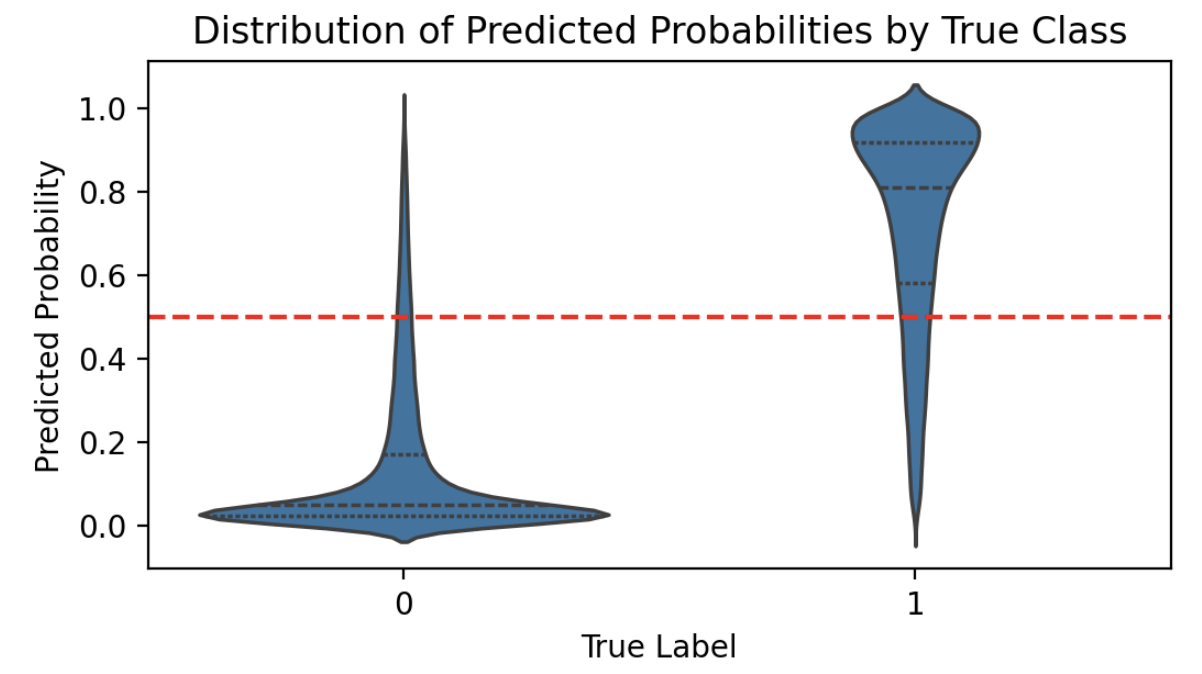
\includegraphics[width=0.5\linewidth]{violin.png}
    \caption{Enter Caption}
    \label{fig:placeholder}
\end{figure}

The following plot is the confusion matrix. The accuracy from this model is 90.8\%. The precision is 84.9\%. The recall is 80.9\%. The F1 score is 82.9\%. The AMIC model is highly accurate overall. The model also has a good balance between precision and recall. The AMIC accuracy without using Monte Carlo samples is 88.42\%. However, once we use Monte Carlo samples to calculate the accuracy, it increases to 91\%. This means that the uncertainty not only helps to provide more measurements but also improves the point estimation. 
\begin{figure}
    \centering
    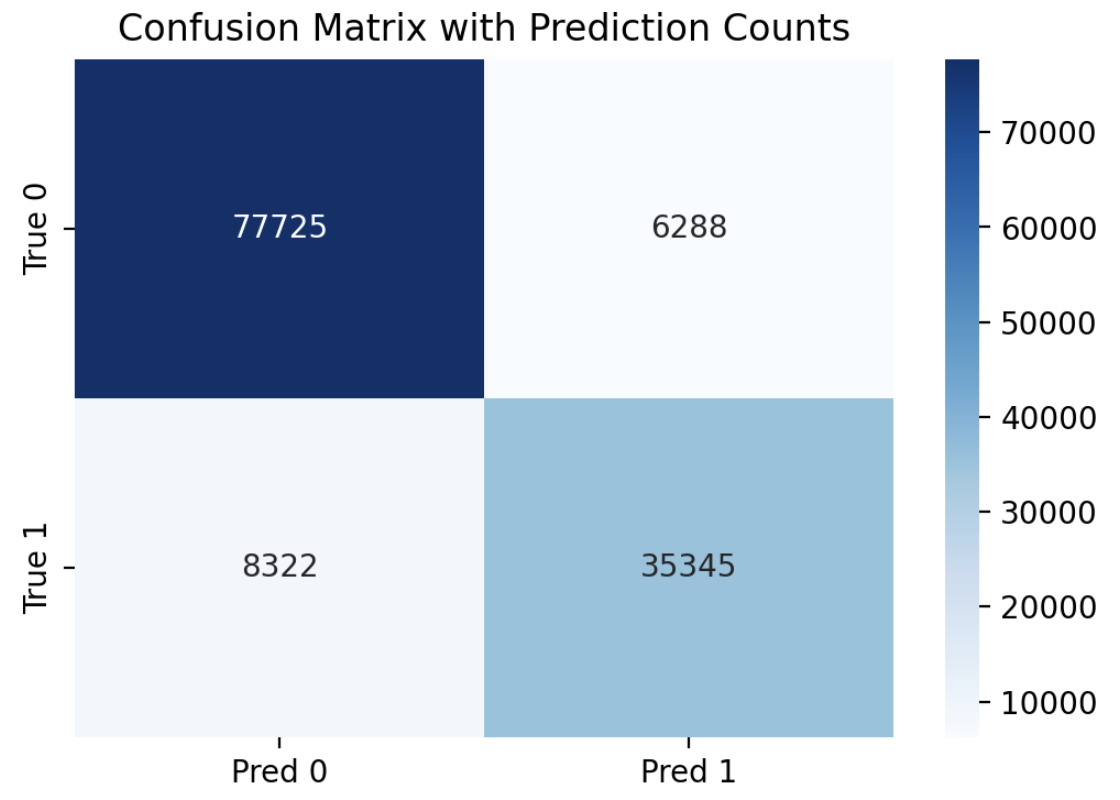
\includegraphics[width=0.5\linewidth]{confusion.png}
    \caption{Confusion Matrix}
    \label{fig:placeholder}
\end{figure}
\end{document}
